\scanpage{10}
3) On vérifie \inserted{\figure{\begin{tikzpicture}[x=1cm,y=1cm,baseline=-.5ex]
\node at (2.9,.55) {par R.R. pour $A\times A\xrightarrow{\pi_A}A$};
\draw (.12,-.22) .. controls (.12,.1) and (-.15,.22) .. (.02,.67) .. controls (.10,1.05) and (.35,1.02) .. (1.05,1.04) -- (4.8,1.04) .. controls (6.05,1.05) and (6.27,.72) .. (5.72,.35) .. controls (4.6,.05) and (1.3,.40) .. (.48,.10) .. controls (.23,.03) and (.25,-.21) .. (.24,-.39);
\end{tikzpicture}}} que l'on a sur $A$
\[
\unsure{\text{a)}|\alpha)}\qquad\operatorname{ch}(x*y)=\operatorname{ch}(x)*\operatorname{ch}(y)\operatorname{Todd}(t_A)
\]
(donc on a
\[
\operatorname{ch}(x*y)=\operatorname{ch}x*\operatorname{ch}y
\]
si $\operatorname{Todd}t_A=1$, p.ex. si $t_A$ est trivial, p.ex. $S$ local).

Considérons d'autre part l'élément \inserted{$D$} de $\operatorname{Gr}^1(A\times A)$\\
défini par $L$, et considérons le $\exp D$, d'où
\[
\psi_D=\varphi_{\exp D}:\operatorname{Gr}^\bullet(A)_{\unsure{\mathbb Q|\mathbf Q}}\mathbin{-}\operatorname{Gr}^\bullet(B)_{\unsure{\mathbb Q|\mathbf Q}}.
\]
\deleted{\deleted{\unsure{Alors}} On a donc, grâce à RR pour $A\times_S B\mathbin{-}B$\\
et \deleted{\unsure{ce qui précède}} (prop. 1
\[
\psi_D(xy)=\psi_D(x)\psi_D(y).
\]
On veut utiliser prop. 2 pour calculer\\
$\psi_D(a*b)$. On a, si
\[
a=\operatorname{ch}x,\qquad b=\operatorname{ch}y
\]
\deleted{$\unsure{*}$} $x*y=\operatorname{ch}a*\operatorname{ch}b=\operatorname{ch}(a*b)T_{\deleted{\unsure{x}}}^{-1}$\qquad $(T=\operatorname{Todd}(t_A))$\\
d'où $\psi_D(x*y)=\psi_D(\operatorname{ch}(a*b)T^{-1})$.}

\margin{\figure{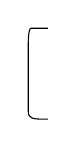
\begin{tikzpicture}[x=.25cm,y=.55cm]\draw (1,2.1)--(.15,2.1)..controls (0,2.1) and (0,1.8)..(0,1.6)--(0,.2)..controls (0,0) and (.2,0)..(1,0);\end{tikzpicture}}}
\deleted{\unsure{Si}} On a, par RR pour $A\times_S B\longrightarrow B$
\[
\operatorname{ch}(\varphi_{\mathcal L}(x))=\psi_D(\operatorname{ch}(\unsure{a|x}))T
\qquad(T=\operatorname{Todd}t_A)
\]
\deleted{\unsure{Supposons} \deleted{\unsure{Posons}} $a=\operatorname{ch}x$}\\
Posons $a=\operatorname{ch}x$, $b=\operatorname{ch}y$, et transformons\\
$\varphi_{\mathcal L}(x*y)=\varphi_{\mathcal L}(x)\varphi_{\mathcal L}(y)$ (prop 1) par $\operatorname{ch}$, on trouve
\[
\psi_D(\operatorname{ch}(x*y))T=\psi_D(\operatorname{ch}(x))T\,\psi_D(\operatorname{ch}(y))T
\]
\deleted{d'où}\\
d'où, \deleted{$\unsure{\varphi}$} grâce à $\unsure{\text{a)}|\alpha)}$
\[
\psi_D(\deleted{\unsure{\operatorname{ch}(x*y)}}\operatorname{ch}x*\operatorname{ch}y)T^2\deleted{\unsure{T}}
=\psi_D(\operatorname{ch}x)\psi_D(\operatorname{ch}y)T^2
\]
d'où
\[
\boxed{\psi_D(\unsure{a|\operatorname{ch}a}*b)=\psi_D(a)\psi_D(b)}
\]
\mspage{9}
